\section{Technika sítí a protokolů - komunikační modely, způsob přenosu informace, základní struktura sítí, typy sítí, architektura komunikace systémů.}

\subsection{Komunikační modely}

Komunikaci mezi dvěma stranami lze rozlišit na~dva typy: \textbf{komunikaci uvnitř sítí} a~\textbf{komunikaci mezi koncovými uživateli} (nad~sítěmi).

\textbf{Data} jsou reprezentace faktů, pojmů nebo instrukcí ve~formální podobě vhodná pro~komunikaci a~interpretaci pro~strojové zpracování. \textbf{Informace} je význam dat, důležitý typicky pro~uživatele.

\begin{figure}[ht]
	\centering
	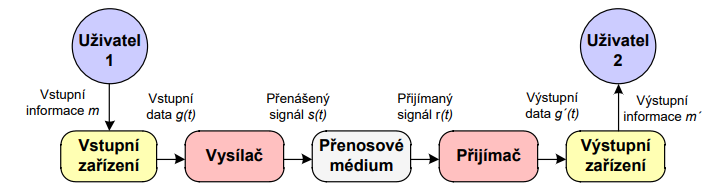
\includegraphics[width=\textwidth]{images/q01_simplified_scheme_network}
	\caption
		[Zjednodušené blokové schéma datovké komunikace]
		{Zjednodušené blokové schéma datovké komunikace. \\
		Informace $m$ je pomocí vstupního zařízení reprentována jako data $g(t)$ ve~formě proměnlivého časového signálu, který musí být přeložen do~podoby vhodné pro~přenosové médium, tj. do~signálu $s(t)$, vysílačem. Na~druhé straně se objeví jako signál $r(t)$, který se od~odeslaného může odlišovat (šum, rušení). Je konvertován zpět do~tvaru výstupních dat $g'(t)$ a~výstupnímu zařízení jsou předána data $m'$.}
	\label{q01_simplified_scheme_network}
\end{figure}

Pomocí komunikačních sítí spolu komunikují koncoví uživatelé, v~případě počítačů partnerské procesy na~komunikujících počítačích. Základním předpokladem pro~komunikaci uživatelů je definice rozhraní mezi~uživatelem a~sítí; musí konkretizovat strukturu a~formát předávaných uživatelských a~řídících dat.

\begin{figure}[ht]
	\centering
	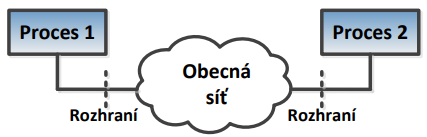
\includegraphics[width=0.5\textwidth]{images/q01_simplified_scheme_processes}
	\caption{Zjednodušené blokové schéma komunikace mezi procesy pracujícími na~samostatných počítačích propojených obecnou sítí.}
	\label{q01_simplified_scheme_processes}
\end{figure}

Základní úkoly pro~přenos informace spočívají ve~vlastním \textbf{přenosu} informace (kódování dat a~jejich přizpůsobení pro~telekomunikační kanál), vyhledání cesty spojení dvou uživatelů v~síti (\textbf{směrování}) a~použití vhodného způsobu komunikace a~řízení (\textbf{protokoly}).

Komunikační řetězec zejména stará o~řízení výměny informací (způsob organizace přenosu dat mezi zdrojem a~cílem informace), definice rozhraní (včetně tvaru a~velikosti signálu), synchronizaci (časové sjednocení), formátování zpráv (unifikace způsobu sestavení obsahu zprávy) a~adresování a~směrování (jednoznačný způsob určení cíle a~nalezení cesty k~němu).

Komunikační řetězec zpravidla umožňuje vícenásobné využití přenosových systémů (sdílení více uživateli/procesy), řízení systému (konfigurace, dohled, reakce na~chyby a~přetížení), detekci a~korelaci chyb, zotavení se ze~ztrát v~komunikačním systému, řízení přenosu (aby nedocházelo k~zahlcení systému nadměrným množstvím dat) a~ochranu zpráv (zaslaná data může přijímat pouze příjemce).

\clearpage
\section{Základní popis referenčního modelu ISO/OSI a srovnání s TCP/IP.}

\clearpage
\section{Základní popis síťového modelu TCP/IP a srovnání s ISO/OSI.}

\clearpage
\section{Principy komunikačních technik -- vícenásobné využití cest, zajištění obousměrné komunikace.}

\clearpage
\section{Fyzická vrstva přenosových systémů -- přenosová média, analogové a digitální modulace, klíčovací techniky, princip digitalizace řečového signálu.}

\clearpage
\section{Spojová vrstva přenosových systémů -- podvrstvy, rámce spojové vrstvy, adresace, metody zajištění spolehlivého přenosu.}

\clearpage
\section{Síťová vrstva přenosových systémů -- spínání paketů, služby síťové vrstvy, IPv4 adresy, techniky směrování, IPv4 datagram.}

\clearpage
\section{Síťová vrstva přenosových systémů -- tunelování paketů, ARP, NAT, ICMPv4, IPv6.}

\clearpage
\section{Transportní vrstva přenosových systémů -- služby transportní vrstvy, UDP protokol, TCP protokol.}

\clearpage
\section{Aplikační vrstva přenosových systémů -- DHCP protokol, DNS systém, přenos souborů, webové protokoly, elektronická pošta.}
